\documentclass[man]{apa6}
\usepackage{lmodern}
\usepackage{amssymb,amsmath}
\usepackage{ifxetex,ifluatex}
\usepackage{fixltx2e} % provides \textsubscript
\ifnum 0\ifxetex 1\fi\ifluatex 1\fi=0 % if pdftex
  \usepackage[T1]{fontenc}
  \usepackage[utf8]{inputenc}
\else % if luatex or xelatex
  \ifxetex
    \usepackage{mathspec}
  \else
    \usepackage{fontspec}
  \fi
  \defaultfontfeatures{Ligatures=TeX,Scale=MatchLowercase}
\fi
% use upquote if available, for straight quotes in verbatim environments
\IfFileExists{upquote.sty}{\usepackage{upquote}}{}
% use microtype if available
\IfFileExists{microtype.sty}{%
\usepackage{microtype}
\UseMicrotypeSet[protrusion]{basicmath} % disable protrusion for tt fonts
}{}
\usepackage{hyperref}
\hypersetup{unicode=true,
            pdftitle={A practical primer on processing semantic property norm data},
            pdfauthor={Erin M. Buchanan, Simon De Deyne, \& Maria Montefinese},
            pdfkeywords={semantic, property norm task, tutorial},
            pdfborder={0 0 0},
            breaklinks=true}
\urlstyle{same}  % don't use monospace font for urls
\usepackage{color}
\usepackage{fancyvrb}
\newcommand{\VerbBar}{|}
\newcommand{\VERB}{\Verb[commandchars=\\\{\}]}
\DefineVerbatimEnvironment{Highlighting}{Verbatim}{commandchars=\\\{\}}
% Add ',fontsize=\small' for more characters per line
\usepackage{framed}
\definecolor{shadecolor}{RGB}{248,248,248}
\newenvironment{Shaded}{\begin{snugshade}}{\end{snugshade}}
\newcommand{\AlertTok}[1]{\textcolor[rgb]{0.94,0.16,0.16}{#1}}
\newcommand{\AnnotationTok}[1]{\textcolor[rgb]{0.56,0.35,0.01}{\textbf{\textit{#1}}}}
\newcommand{\AttributeTok}[1]{\textcolor[rgb]{0.77,0.63,0.00}{#1}}
\newcommand{\BaseNTok}[1]{\textcolor[rgb]{0.00,0.00,0.81}{#1}}
\newcommand{\BuiltInTok}[1]{#1}
\newcommand{\CharTok}[1]{\textcolor[rgb]{0.31,0.60,0.02}{#1}}
\newcommand{\CommentTok}[1]{\textcolor[rgb]{0.56,0.35,0.01}{\textit{#1}}}
\newcommand{\CommentVarTok}[1]{\textcolor[rgb]{0.56,0.35,0.01}{\textbf{\textit{#1}}}}
\newcommand{\ConstantTok}[1]{\textcolor[rgb]{0.00,0.00,0.00}{#1}}
\newcommand{\ControlFlowTok}[1]{\textcolor[rgb]{0.13,0.29,0.53}{\textbf{#1}}}
\newcommand{\DataTypeTok}[1]{\textcolor[rgb]{0.13,0.29,0.53}{#1}}
\newcommand{\DecValTok}[1]{\textcolor[rgb]{0.00,0.00,0.81}{#1}}
\newcommand{\DocumentationTok}[1]{\textcolor[rgb]{0.56,0.35,0.01}{\textbf{\textit{#1}}}}
\newcommand{\ErrorTok}[1]{\textcolor[rgb]{0.64,0.00,0.00}{\textbf{#1}}}
\newcommand{\ExtensionTok}[1]{#1}
\newcommand{\FloatTok}[1]{\textcolor[rgb]{0.00,0.00,0.81}{#1}}
\newcommand{\FunctionTok}[1]{\textcolor[rgb]{0.00,0.00,0.00}{#1}}
\newcommand{\ImportTok}[1]{#1}
\newcommand{\InformationTok}[1]{\textcolor[rgb]{0.56,0.35,0.01}{\textbf{\textit{#1}}}}
\newcommand{\KeywordTok}[1]{\textcolor[rgb]{0.13,0.29,0.53}{\textbf{#1}}}
\newcommand{\NormalTok}[1]{#1}
\newcommand{\OperatorTok}[1]{\textcolor[rgb]{0.81,0.36,0.00}{\textbf{#1}}}
\newcommand{\OtherTok}[1]{\textcolor[rgb]{0.56,0.35,0.01}{#1}}
\newcommand{\PreprocessorTok}[1]{\textcolor[rgb]{0.56,0.35,0.01}{\textit{#1}}}
\newcommand{\RegionMarkerTok}[1]{#1}
\newcommand{\SpecialCharTok}[1]{\textcolor[rgb]{0.00,0.00,0.00}{#1}}
\newcommand{\SpecialStringTok}[1]{\textcolor[rgb]{0.31,0.60,0.02}{#1}}
\newcommand{\StringTok}[1]{\textcolor[rgb]{0.31,0.60,0.02}{#1}}
\newcommand{\VariableTok}[1]{\textcolor[rgb]{0.00,0.00,0.00}{#1}}
\newcommand{\VerbatimStringTok}[1]{\textcolor[rgb]{0.31,0.60,0.02}{#1}}
\newcommand{\WarningTok}[1]{\textcolor[rgb]{0.56,0.35,0.01}{\textbf{\textit{#1}}}}
\usepackage{graphicx,grffile}
\makeatletter
\def\maxwidth{\ifdim\Gin@nat@width>\linewidth\linewidth\else\Gin@nat@width\fi}
\def\maxheight{\ifdim\Gin@nat@height>\textheight\textheight\else\Gin@nat@height\fi}
\makeatother
% Scale images if necessary, so that they will not overflow the page
% margins by default, and it is still possible to overwrite the defaults
% using explicit options in \includegraphics[width, height, ...]{}
\setkeys{Gin}{width=\maxwidth,height=\maxheight,keepaspectratio}
\IfFileExists{parskip.sty}{%
\usepackage{parskip}
}{% else
\setlength{\parindent}{0pt}
\setlength{\parskip}{6pt plus 2pt minus 1pt}
}
\setlength{\emergencystretch}{3em}  % prevent overfull lines
\providecommand{\tightlist}{%
  \setlength{\itemsep}{0pt}\setlength{\parskip}{0pt}}
\setcounter{secnumdepth}{0}
% Redefines (sub)paragraphs to behave more like sections
\ifx\paragraph\undefined\else
\let\oldparagraph\paragraph
\renewcommand{\paragraph}[1]{\oldparagraph{#1}\mbox{}}
\fi
\ifx\subparagraph\undefined\else
\let\oldsubparagraph\subparagraph
\renewcommand{\subparagraph}[1]{\oldsubparagraph{#1}\mbox{}}
\fi

%%% Use protect on footnotes to avoid problems with footnotes in titles
\let\rmarkdownfootnote\footnote%
\def\footnote{\protect\rmarkdownfootnote}


  \title{A practical primer on processing semantic property norm data}
    \author{Erin M. Buchanan\textsuperscript{1}, Simon De Deyne\textsuperscript{2}, \& Maria Montefinese\textsuperscript{3}}
    \date{}
  
\shorttitle{Processing Norms}
\affiliation{
\vspace{0.5cm}
\textsuperscript{1} Harrisburg University of Science and Technology\\\textsuperscript{2} The University of Melbourne\\\textsuperscript{3} University of Padua}
\keywords{semantic, property norm task, tutorial}
\usepackage{csquotes}
\usepackage{upgreek}
\captionsetup{font=singlespacing,justification=justified}

\usepackage{longtable}
\usepackage{lscape}
\usepackage{multirow}
\usepackage{tabularx}
\usepackage[flushleft]{threeparttable}
\usepackage{threeparttablex}

\newenvironment{lltable}{\begin{landscape}\begin{center}\begin{ThreePartTable}}{\end{ThreePartTable}\end{center}\end{landscape}}

\makeatletter
\newcommand\LastLTentrywidth{1em}
\newlength\longtablewidth
\setlength{\longtablewidth}{1in}
\newcommand{\getlongtablewidth}{\begingroup \ifcsname LT@\roman{LT@tables}\endcsname \global\longtablewidth=0pt \renewcommand{\LT@entry}[2]{\global\advance\longtablewidth by ##2\relax\gdef\LastLTentrywidth{##2}}\@nameuse{LT@\roman{LT@tables}} \fi \endgroup}


\DeclareDelayedFloatFlavor{ThreePartTable}{table}
\DeclareDelayedFloatFlavor{lltable}{table}
\DeclareDelayedFloatFlavor*{longtable}{table}
\makeatletter
\renewcommand{\efloat@iwrite}[1]{\immediate\expandafter\protected@write\csname efloat@post#1\endcsname{}}
\makeatother
\usepackage{lineno}

\linenumbers

\authornote{

Correspondence concerning this article should be addressed to Erin M. Buchanan, 326 Market St., Harrisburg, PA 17101. E-mail: \href{mailto:ebuchanan@harrisburgu.edu}{\nolinkurl{ebuchanan@harrisburgu.edu}}}

\abstract{
Semantic property listing tasks require participants to generate short propositions (e.g., \textless{}\emph{barks}\textgreater{}, \textless{}\emph{has fur}\textgreater{}) for a specific concept (e.g., dog). This task is the cornerstone of the creation of semantic property norms which are essential for modelling, stimuli creation, and understanding similarity between concepts. However, despite the wide applicability of semantic property norms for a large variety of concepts across different groups of people, the methodological aspects of the property listing task have received less attention, even though the procedure and processing of the data can substantially affect the nature and quality of the measures derived from them. The goal of this paper is to provide a practical primer on how to collect and process semantic property norms. We will discuss the key methods to elicit semantic properties and compare different methods to derive meaningful representations from them. This will cover the role of instructions and test context, property pre-processing (e.g., lemmatization), property weighting, and relationship encoding using ontologies. With these choices in mind, we propose and demonstrate a processing pipeline that transparently documents these steps resulting in improved comparability across different studies. The impact of these choices will be demonstrated using intrinsic (e.g., reliability, number of properties) and extrinsic measures (e.g., categorization, semantic similarity, lexical processing). This practical primer will offer potential solutions to several longstanding problems and allow researchers to develop new property listing norms overcoming the constraints of previous studies.


}

\begin{document}
\maketitle

Semantic properties are assumed to be, entirely or in part, the building blocks of semantic representation -- the knowledge we have of the world - by a variety of theories (e.g., Collins \& Quillian, 1969, @Jackendoff; Jackendoff, 1992; Minsky, 1975; Norman \& Rumelhart, 1975; Saffran \& Sholl, 1999; Smith \& Medin, 1981) and computational models (Caramazza, Laudanna, \& Romani, 1988; Farah \& McClelland, 1991; Humphreys \& Forde, 2001). Within this perspective, the meaning of a concept is conceived as a distributed pattern of semantic properties, which convey multiple types of information (Cree \& McRae, 2003; Plaut, 2002; Rogers et al., 2004). For example, the concept HORSE can be described by encyclopedic (\textless{}\emph{is a mammal}\textgreater{}), visual (\textless{}\emph{is furry}\textgreater{}, \textless{}\emph{has legs}\textgreater{}, \textless{}\emph{has a tail}\textgreater{}, \textless{}\emph{has a mane}\textgreater{}), functional (\textless{}\emph{used for racing}\textgreater{}), and motor (\textless{}\emph{gallops}\textgreater{}) information. Given the relevance of semantic properties in shaping theories of semantic representation, researchers have recognized the value of collecting semantic property production norms. Typically, in the property generation task, participants are presented with a set of concepts and are asked to list the properties they think are characteristic for each concept meaning. Generally, in this task, the concepts are called \emph{cues}, and the responses to the cue are called \emph{features}\footnote{Throughout this article, features will be distinguished from cues using angular brackets.}. This method has a long history of use by researchers wishing to gain insight into semantic representations of concrete concepts and categories (McRae, Cree, Seidenberg, \& McNorgan, 2005; Rosch \& Mervis, 1975; Smith, Shoben, \& Rips, 1974), and more recently, events and abstract concepts (Lebani, Lenci, \& Bondielli, 2016; Vinson \& Vigliocco, 2008; Wiemer-Hastings \& Xu, 2005).

On the one hand, many studies adopted the property generation task itself to make inferences about word meaning and its computation (Recchia \& Jones, 2012; Santos, Chaigneau, Simmons, \& Barsalou, 2011; Wiemer-Hastings \& Xu, 2005; Wu \& Barsalou, 2009). On the other hand, researchers employed the property listing task in order to provide other researchers with a tool of standardized word stimuli and relative semantic measures. Indeed, based on data obtained from the property production task, it is then possible to calculate numerous measures and distributional statistics both at the feature and the concept level. For example, these feature data can be used to determine the semantic similarity/distance between concepts, often by calculating the feature overlap or number of shared features between concepts (Buchanan, Valentine, \& Maxwell, 2019; McRae et al., 2005; Montefinese, 2019; Montefinese, Zannino, \& Ambrosini, 2015; Vigliocco, Vinson, Lewis, \& Garrett, 2004), or how different types (Daniele Zannino, Perri, Pasqualetti, Caltagirone, \& Carlesimo, 2006; Kremer \& Baroni, 2011) and dimensions of feature informativeness, such as, distinctiveness (Garrard, Lambon Ralph, Hodges, \& Patterson, 2001), cue validity (Rosch \& Mervis, 1975), relevance (Sartori \& Lombardi, 2004), semantic richness (Pexman, Hargreaves, Siakaluk, Bodner, \& Pope, 2008), and significance (Montefinese, Ambrosini, Fairfield, \& Mammarella, 2014) are distributed across concepts.

Efficient ways to collect data online have boosted the availability of large feature listing data sets. These semantic feature norms are now available across different languages: Dutch (De Deyne \& Storms, 2008; Ruts et al., 2004), English (Buchanan, Holmes, Teasley, \& Hutchison, 2013; Buchanan et al., 2019; Devereux, Tyler, Geertzen, \& Randall, 2014; Garrard et al., 2001; McRae et al., 2005; Vinson \& Vigliocco, 2008), German (Kremer \& Baroni, 2011), Italian (Catricalà et al., 2015; Kremer \& Baroni, 2011; Montefinese, Ambrosini, Fairfield, \& Mammarella, 2013; Zannino, Perri, Pasqualetti, Caltagirone, \& Carlesimo, 2006), Portuguese (Marques, Fonseca, Morais, \& Pinto, 2007), and Spanish (Vivas, Vivas, Comesaña, Coni, \& Vorano, 2017) as well as for blind participants (Lenci, Baroni, Cazzolli, \& Marotta, 2013). However, these norms vary substantially in the procedure of data collection and their pre-processing, and this does not facilitate performing cross-language comparisons and, thus, making inferences about how semantic representations are generalizable across languages.

First, there is a lack of agreement in the instructions provided to the participants. Indeed, while some studies use an open-ended verbal feature production (Buchanan et al., 2013, 2019; De Deyne \& Storms, 2008; Montefinese et al., 2013) where participants can list the features related to the concept with any kind of semantic relation, other studies use a constrained verbal feature production (Devereux et al., 2014; Garrard et al., 2001) where participants were instructed to use specific semantic relations between cue concept and features, such as, for example, \textless{}\emph{is \ldots{}}\textgreater{}, \textless{}\emph{has \ldots{}}\textgreater{}, \textless{}\emph{does \ldots{}}\textgreater{}, \textless{}\emph{made of \ldots{}}\textgreater{}, and so forth. Moreover, some authors instruct the participants to produce a single word as a feature instead of a multiple-word description. This latter case could also determine a problem on subsequent coding steps that affect the identification of pieces of information. For example, if the participant listed the feature \textless{}\emph{has four wheels}\textgreater{} for the concept CAR, there is no consensus if this feature should be divided into \textless{}\emph{has wheels}\textgreater{} and \textless{}\emph{has four wheels}\textgreater{}, under the assumption that the participant provided two bits of information, or rather if it should be considered as a unique feature. Second, some authors gave a time limit to provide the features descriptions (Kremer \& Baroni, 2011; Lenci et al., 2013; Marques et al., 2007) or a limited number of features to be listed (De Deyne \& Storms, 2008), with a possible influence on a number of feature-based measures (e.g., semantic richness or distinctiveness).

Because the feature listing task is a verbal task and language is very productive (i.e., the same feature can be expressed in many different ways), few features will be listed in exactly the same way across participants. To be able to derive reliable quantitative measures, nearly all studies specify a series of pre-processing steps to group verbal utterances about the same underlying conceptual property together. The main problem is that there is no agreement about how to code/pre-process data derived from the feature listing task. Recoding features is sometimes done in manually (McRae et al., 2005) whereas others use semi-automatic procedures, especially for larger datasets (Buchanan et al., 2019). Further points of debate are related to the inclusion/exclusion of certain types of responses. For example, unlike previous semantic norms (McRae et al., 2005; Montefinese et al., 2013; Vivas et al., 2017), Buchanan et al. (2019) included idiosyncratic features (features produced only by one or a few number of participants) if they were in the top listed features, ambiguous words (words with multiple meanings), and created a special coding for affixes of the root words. Moreover, they discarded stop words, such as, the, an, of, and synonyms were treated as different entries.

While hand-coding features leads to features that concise, easily interpretable, and highly predictive of semantic behavior, the increasing scale of recent studies and more powerful natural language processing techniques make automatic procedures an attractive alternative. Moreover, building standard automatic procedures to process feature-listing data would not only add transparency to the process but would also prevent human errors and allow a generalization of the data across languages. For the first time, in this study we propose an automatic procedure to code the raw feature data derived from a semantic feature listing task (SFL). The next sections provide a tutorial on how raw feature data might be processed to a more compact feature output. The tutorial is written for \emph{R} and is fully documented, such that users can adapt it to their language of choice (\url{https://github.com/doomlab/FLT-Primer}). Figure \ref{fig:flowchart} portrays the proposed set of steps including spell checking, lemmatization, exclusion of stop words, and final processing in a multi-word sequence approach or a bag of words approach. After detailing these steps, the final data form will evaluated and compared to previous norms to determine the usefulness of this approach.

\begin{figure}
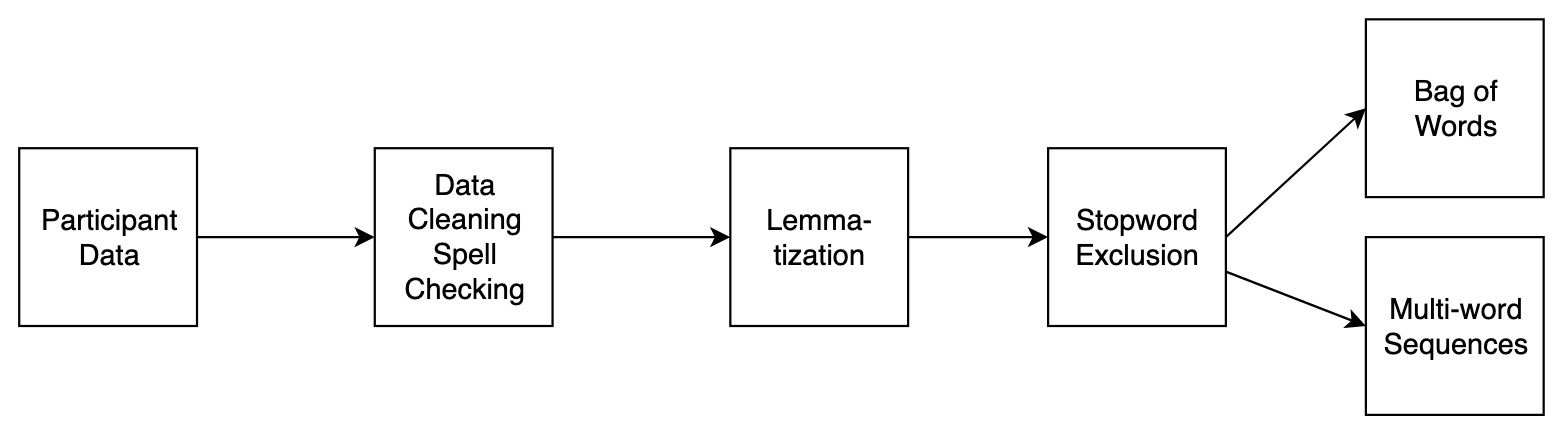
\includegraphics[width=5.24in]{flow_chart} \caption{Flow chart illustrating how feature listings are recoded to obtain a standard feature format.}\label{fig:flowchart}
\end{figure}

\hypertarget{materials-and-data-format}{%
\subsection{Materials and Data Format}\label{materials-and-data-format}}

You can load the entire set of libraries for this tutorial as shown below using \texttt{dependencies.R} found online\footnote{A \texttt{packrat} project compilation is available on GitHub for reproducibility (Ushey, McPherson, Cheng, Atkins, \& Allaire, 2018)}.

\scriptsize

\begin{Shaded}
\begin{Highlighting}[]
\KeywordTok{library}\NormalTok{(here)}
\KeywordTok{library}\NormalTok{(dplyr)}
\CommentTok{#Spelling}
\KeywordTok{library}\NormalTok{(hunspell)}
\KeywordTok{library}\NormalTok{(tidytext)}
\KeywordTok{library}\NormalTok{(stringi)}
\CommentTok{#Lemmatization}
\KeywordTok{library}\NormalTok{(koRpus) }
\KeywordTok{library}\NormalTok{(koRpus.lang.en)}
\KeywordTok{library}\NormalTok{(tokenizers)}
\CommentTok{#Stopwords}
\KeywordTok{library}\NormalTok{(stopwords)}
\end{Highlighting}
\end{Shaded}

\normalsize

The data can then be imported with \texttt{importData.R}. Additionally, the answers from participants may need to be normalized into lowercase for consistency.

\scriptsize

\begin{Shaded}
\begin{Highlighting}[]
\CommentTok{# Importing the raw feature lists}
\NormalTok{X <-}\StringTok{ }\KeywordTok{read.csv}\NormalTok{(}\StringTok{"../raw_data/tidy_words.csv"}\NormalTok{, }\DataTypeTok{stringsAsFactors =}\NormalTok{ F)}
\CommentTok{## Lower case to normalize}
\NormalTok{X}\OperatorTok{$}\NormalTok{answer <-}\StringTok{ }\KeywordTok{tolower}\NormalTok{(X}\OperatorTok{$}\NormalTok{answer)}
\end{Highlighting}
\end{Shaded}

\normalsize

\begin{table}[t]

\caption{\label{tab:tab1}Example of Data Formatted for Tidy Data}
\centering
\begin{tabular}{l>{\raggedright\arraybackslash}p{30em}}
\toprule
word & answer\\
\midrule
airplane & you fly in it  its big  it is fast  they are expensive  they are at an airport  you have to be trained to fly it  there are lots of seats  they get very high up\\
airplane & wings engine pilot cockpit tail\\
airplane & wings  it flys  modern technology  has passengers  requires a pilot  can be dangerous  runs on gas  used for travel\\
airplane & wings  flys  pilot  cockpit  uses gas  faster travel\\
airplane & wings  engines  passengers  pilot(s)  vary in size and color\\
\addlinespace
airplane & wings  body  flies  travel\\
\bottomrule
\end{tabular}
\end{table}

The data for this tutorial includes 16544 unique concept-feature responses for 226 concepts from Buchanan et al. (2019). The concepts were taken from McRae et al. (2005), Vinson and Vigliocco (2008), and Bruni, Tran, and Baroni (2014). The concepts include 185 nouns, 25 verbs, and 16 adjectives. Concreteness ratings collected by Brysbaert, Warriner, and Kuperman (2014) were matched with the current data set. The concreteness ratings capture the difference between abstract (language-based) and concrete (experience-based) concepts and were measured on a five-point scale. Nouns were rated as most concrete: \emph{M} = 4.59 (\emph{SD} = 0.52), followed by adjectives: \emph{M} = 3.78 (\emph{SD} = 0.81), and verbs: \emph{M} = 3.57 (\emph{SD} = 0.79). The SFL data consist of a text file where concept-feature observation is a row and each column is a variable. An example of these raw data are shown in Table \ref{tab:tab1}, where the \texttt{word} column is the cue, and the \texttt{answer} column denotes a single participant's response. The original data can be found at \url{https://osf.io/cjyzw/}.

The data was collected using the instructions provided by McRae et al. (2005), however, in contrast to the suggestions for consistency detailed above (Devereux et al., 2014), each participant was simply given a large text box to include their answer. Each answer includes multiple embedded features, and the tutorial proceeds to demonstrate potential processing addressing the data in this nature. With structured data entry for participants (e.g., asking participants to type one feature on each line), the suggested processing steps are reduced.

\hypertarget{spelling}{%
\subsection{Spelling}\label{spelling}}

The first step (see Figure \ref{fig:flowchart}) in processing the features consists of identifying and replacing spelling mistakes. Spell checking can be automated with the \texttt{hunspell} package in \emph{R} (Ooms, 2018) using \texttt{spellCheck.R}. Each \texttt{answer} can be checked for misspellings across an entire column of answers, which is in the \texttt{X} dataset. Because participants were recruited in the United States, we used the default American English dictionary. The \texttt{hunspell} vignettes provide details on how to import your own dictionary for non-English languages. The choice of dictionary should also normalize between multiple varieties of the same language, for example, the \texttt{"en\_GB"} would convert to British English spellings.

\scriptsize

\begin{Shaded}
\begin{Highlighting}[]
\CommentTok{# Extract a list of words}
\NormalTok{tokens =}\StringTok{ }\KeywordTok{unnest_tokens}\NormalTok{(}\DataTypeTok{tbl =}\NormalTok{ X, }\DataTypeTok{output =}\NormalTok{ token, }\DataTypeTok{input =}\NormalTok{ answer)}
\NormalTok{wordlist =}\StringTok{ }\KeywordTok{unique}\NormalTok{(tokens}\OperatorTok{$}\NormalTok{token)}
\CommentTok{# Spell check the words}
\NormalTok{spelling.errors <-}\StringTok{ }\KeywordTok{hunspell}\NormalTok{(wordlist)}
\NormalTok{spelling.errors <-}\StringTok{ }\KeywordTok{unique}\NormalTok{(}\KeywordTok{unlist}\NormalTok{(spelling.errors))}
\NormalTok{spelling.sugg <-}\StringTok{ }\KeywordTok{hunspell_suggest}\NormalTok{(spelling.errors, }\DataTypeTok{dict =} \KeywordTok{dictionary}\NormalTok{(}\StringTok{"en_US"}\NormalTok{))}
\end{Highlighting}
\end{Shaded}

\normalsize

The result from the \texttt{hunspell()} function is a list object of spelling errors for each row of data. For example, when responding to APPLE, a participant wrote \textless{}\emph{fruit grocery store orchard red green yelloe good with peanut butter good with caramell}\textgreater{}, and the spelling errors were denoted as \textless{}\emph{yelloe\textgreater{} \textless{}caramell}\textgreater{}. After checking for errors, the \texttt{hunspell\_suggest()} function was used to determine the most likely replacement for each error. For \textless{}\emph{yelloe}\textgreater{}, both \textless{}\emph{yellow\textgreater{} \textless{}yell}\textgreater{} were suggested, and \textless{}\emph{caramel\textgreater{} \textless{}camel}\textgreater{} were suggested for \textless{}\emph{caramell}\textgreater{}.

Answers are provided in the most probable order, therefore, the first suggestion is selected as the correct answer. These answers are compiled into a spelling dictionary, which is saved for reproducibility. In addition to the hunspell dictionary, an auxiliary dictionary with pre-coded error responses and corrections could also be added at this stage to catch any false positives by adding entries to the \texttt{spelling.dict}. Other paid alternatives, such as Bing Spell Check, can be a useful avenue for datasets that may contain brand names (i.e, \emph{apple} versus \emph{Apple}) or slang terms and provides context sensitive corrections (e.g., keeping \emph{Apple} as a response to computer, but not as a response to green).

\scriptsize

\begin{Shaded}
\begin{Highlighting}[]
\CommentTok{# Pick the first suggestion}
\NormalTok{spelling.sugg <-}\StringTok{ }\KeywordTok{unlist}\NormalTok{(}\KeywordTok{lapply}\NormalTok{(spelling.sugg, }\ControlFlowTok{function}\NormalTok{(x) x[}\DecValTok{1}\NormalTok{]))}
\NormalTok{spelling.dict <-}\StringTok{ }\KeywordTok{as.data.frame}\NormalTok{(}\KeywordTok{cbind}\NormalTok{(spelling.errors,spelling.sugg))}
\NormalTok{spelling.dict}\OperatorTok{$}\NormalTok{spelling.pattern <-}\StringTok{ }\KeywordTok{paste0}\NormalTok{(}\StringTok{"}\CharTok{\textbackslash{}\textbackslash{}}\StringTok{b"}\NormalTok{, spelling.dict}\OperatorTok{$}\NormalTok{spelling.errors, }\StringTok{"}\CharTok{\textbackslash{}\textbackslash{}}\StringTok{b"}\NormalTok{)}
\CommentTok{# Write out spelling dictionary}
\KeywordTok{write.csv}\NormalTok{(}\DataTypeTok{x =}\NormalTok{ spelling.dict, }\DataTypeTok{file =} \StringTok{"../output_data/spelling.dict.csv"}\NormalTok{, }
          \DataTypeTok{fileEncoding =} \StringTok{"utf8"}\NormalTok{, }\DataTypeTok{row.names =}\NormalTok{ F)}
\end{Highlighting}
\end{Shaded}

\normalsize

As noted, data was collected with a large text box, allowing participants to free respond to the target cue. Participants often used extra spacing, tabs or other punctuation to denote separate answers to the cue. The \texttt{unnest\_tokens()} function from \texttt{tidytext} can be used to split their answers into separate response lines and \texttt{trimws()} to remove all extra white spaces (De Queiroz et al., 2019).

\scriptsize

\begin{Shaded}
\begin{Highlighting}[]
\CommentTok{# Parse features}
\NormalTok{tokens <-}\StringTok{ }\KeywordTok{unnest_tokens}\NormalTok{(}\DataTypeTok{tbl =}\NormalTok{ X, }\DataTypeTok{output =}\NormalTok{ token, }
                        \DataTypeTok{input =}\NormalTok{ answer, }\DataTypeTok{token =}\NormalTok{ stringr}\OperatorTok{::}\NormalTok{str_split, }
                        \DataTypeTok{pattern =} \StringTok{"  |}\CharTok{\textbackslash{}\textbackslash{}}\StringTok{, |}\CharTok{\textbackslash{}\textbackslash{}}\StringTok{.|}\CharTok{\textbackslash{}\textbackslash{}}\StringTok{,|}\CharTok{\textbackslash{}\textbackslash{}}\StringTok{;"}\NormalTok{)}
\NormalTok{tokens}\OperatorTok{$}\NormalTok{token <-}\StringTok{ }\KeywordTok{trimws}\NormalTok{(tokens}\OperatorTok{$}\NormalTok{token, }
                       \DataTypeTok{which =} \KeywordTok{c}\NormalTok{(}\StringTok{"both"}\NormalTok{, }\StringTok{"left"}\NormalTok{, }\StringTok{"right"}\NormalTok{), }
                       \DataTypeTok{whitespace =} \StringTok{"[ }\CharTok{\textbackslash{}t\textbackslash{}r\textbackslash{}n}\StringTok{]"}\NormalTok{)}
\end{Highlighting}
\end{Shaded}

\normalsize

To finalize our data cleaning, we can remove blank lines, and use \texttt{stri\_replace\_all\_regex()} is used to replace the spelling errors with their corrections from the \texttt{stringi} package (Gagolewski \& Tartanus, 2019). The spell checked dataframe is then output to a comma delimited file to preserve each workflow step.

\scriptsize

\begin{Shaded}
\begin{Highlighting}[]
\CommentTok{# Remove empty features}
\NormalTok{tokens <-}\StringTok{ }\NormalTok{tokens[}\OperatorTok{!}\NormalTok{tokens}\OperatorTok{$}\NormalTok{token }\OperatorTok{==}\StringTok{""}\NormalTok{,]}
\NormalTok{tokens}\OperatorTok{$}\NormalTok{corrected <-}\StringTok{ }\KeywordTok{stri_replace_all_regex}\NormalTok{(}\DataTypeTok{str =}\NormalTok{ tokens}\OperatorTok{$}\NormalTok{token,}
                                          \DataTypeTok{pattern =}\NormalTok{ spelling.dict}\OperatorTok{$}\NormalTok{spelling.pattern,}
                                          \DataTypeTok{replacement =}\NormalTok{ spelling.dict}\OperatorTok{$}\NormalTok{spelling.sugg,}
                                          \DataTypeTok{vectorize_all =} \OtherTok{FALSE}\NormalTok{)}
\CommentTok{# Rename columns}
\NormalTok{tokens <-}\StringTok{ }\NormalTok{tokens }\OperatorTok\StringTok{ }
\StringTok{  }\KeywordTok{rename}\NormalTok{(}\DataTypeTok{cue =}\NormalTok{ word,}\DataTypeTok{feature =}\NormalTok{ corrected) }\OperatorTok\StringTok{ }
\StringTok{  }\KeywordTok{select}\NormalTok{(cue, feature)}
\CommentTok{# Write processed file}
\KeywordTok{write.csv}\NormalTok{(}\DataTypeTok{x =}\NormalTok{ tokens,}\DataTypeTok{file =} \StringTok{"../output_data/spellchecked.features.csv"}\NormalTok{,}
          \DataTypeTok{fileEncoding =} \StringTok{"utf8"}\NormalTok{,}\DataTypeTok{row.names =}\NormalTok{ F)}
\end{Highlighting}
\end{Shaded}

\normalsize

\hypertarget{lemmatization}{%
\subsection{Lemmatization}\label{lemmatization}}

The next step groups different word forms that share the same lemma. The process of lemmatizing words uses a trained dictionary to convert all tokens part of a a lexeme set (i.e., all words forms that have the same meaning, \emph{am, are, is}) to a common lemma (i.e., \emph{be})\footnote{We mainly focus on lemmatization and do not proceed stemming the word because it introduces additional ambiguity. More specifically, stemming involves processing words using heuristics to remove affixes or inflections, such as \emph{ing} or \emph{s}. The stem or root word may not reflect an actual word in the language, as simply removing an affix does not necessarily produce the lemma. For example, in response to AIRPLANE, \textless{}\emph{flying}\textgreater{} can be easily converted to \textless{}\emph{fly}\textgreater{} by removing the \emph{ing} inflection. However, this same heuristic converts the feature \textless{}\emph{wings}\textgreater{} into \textless{}\emph{w}\textgreater{} after removing both the \emph{s} for a plural marker and the \emph{ing} participle marker.}. Lemmatization is performed using the \texttt{TreeTagger} program (Schmid, 1994) and implemented through the \texttt{koRpus} package in \emph{R} (Michalke, 2018). TreeTagger is a trained tagger designed to annotate part of speech and lemma information in text, and parameter files are available for multiple languages. We will create a unique set of tokenized words to lemmatize to speed computation, as shown in \texttt{lemmatization.R}.

\scriptsize

\begin{Shaded}
\begin{Highlighting}[]
\CommentTok{# Open the spell checked data}
\NormalTok{X <-}\StringTok{ }\KeywordTok{read.csv}\NormalTok{(}\StringTok{"../output_data/spellchecked.features.csv"}\NormalTok{, }\DataTypeTok{stringsAsFactors =}\NormalTok{ F)}
\CommentTok{# Extract the list of updated tokens}
\NormalTok{tokens <-}\StringTok{ }\KeywordTok{unnest_tokens}\NormalTok{(}\DataTypeTok{tbl =}\NormalTok{ X, }\DataTypeTok{output =}\NormalTok{ word, }\DataTypeTok{input =}\NormalTok{ feature)}
\NormalTok{cuelist <-}\StringTok{ }\KeywordTok{unique}\NormalTok{(tokens}\OperatorTok{$}\NormalTok{cue)}
\end{Highlighting}
\end{Shaded}

\normalsize

The \texttt{treetag()} function calls the installation of TreeTagger to provide part of speech tags and lemmas for each token. Importantly, the \texttt{path} option should be the directory of the TreeTagger installation.

\scriptsize

\begin{Shaded}
\begin{Highlighting}[]
\CommentTok{# Create a dataframe for lemmas}
\NormalTok{tokens.tagged <-}\StringTok{ }\KeywordTok{data.frame}\NormalTok{(}\DataTypeTok{doc_id=}\KeywordTok{character}\NormalTok{(),}
                          \DataTypeTok{token=}\KeywordTok{character}\NormalTok{(),}
                          \DataTypeTok{wclass=}\KeywordTok{character}\NormalTok{(),}
                          \DataTypeTok{lemma=}\KeywordTok{character}\NormalTok{(),}
                          \DataTypeTok{stringsAsFactors=}\OtherTok{FALSE}\NormalTok{)}
\CommentTok{# Loop over cues and create lemmas + POS tags }
\ControlFlowTok{for}\NormalTok{ (i }\ControlFlowTok{in} \DecValTok{1}\OperatorTok{:}\KeywordTok{length}\NormalTok{(cuelist))\{}
\NormalTok{  temp.tag <-}\StringTok{ }\KeywordTok{suppressWarnings}\NormalTok{(}
    \KeywordTok{suppressMessages}\NormalTok{(}
      \KeywordTok{treetag}\NormalTok{(}\KeywordTok{c}\NormalTok{(X}\OperatorTok{$}\NormalTok{feature[X}\OperatorTok{$}\NormalTok{cue }\OperatorTok{==}\StringTok{ }\NormalTok{cuelist[i]], }\StringTok{"NULL"}\NormalTok{),}
              \DataTypeTok{treetagger=}\StringTok{"manual"}\NormalTok{, }\DataTypeTok{format=}\StringTok{"obj"}\NormalTok{,}
              \DataTypeTok{TT.tknz=}\OtherTok{FALSE}\NormalTok{, }\DataTypeTok{lang=}\StringTok{"en"}\NormalTok{, }\DataTypeTok{doc_id =}\NormalTok{ cuelist[i],}
              \CommentTok{# These parameters are based on your computer}
              \DataTypeTok{TT.options=}\KeywordTok{list}\NormalTok{(}\DataTypeTok{path=}\StringTok{"~/TreeTagger"}\NormalTok{, }\DataTypeTok{preset=}\StringTok{"en"}\NormalTok{))))}
\NormalTok{  temp.tag <-}\StringTok{ }\NormalTok{temp.tag}\OperatorTok{@}\NormalTok{TT.res }\OperatorTok\StringTok{ }
\StringTok{    }\KeywordTok{mutate_if}\NormalTok{(is.factor, as.character)}
\NormalTok{  tokens.tagged <-}\StringTok{ }\NormalTok{tokens.tagged }\OperatorTok\StringTok{ }
\StringTok{    }\KeywordTok{bind_rows}\NormalTok{(temp.tag }\OperatorTok\StringTok{ }
\StringTok{                }\KeywordTok{select}\NormalTok{(doc_id, token, wclass, lemma))}
\NormalTok{  \}}
\end{Highlighting}
\end{Shaded}

\normalsize

This function returns a tagged corpus object, which can be converted into a dataframe of the token-lemma information. TreeTagger will return \texttt{\textless{}unknown\textgreater{}} for unknown values and \texttt{@card@} for numbers, and these values were replaced with the original token. Table \ref{tab:tab2} portrays example results from TreeTagger.

\scriptsize

\begin{Shaded}
\begin{Highlighting}[]
\NormalTok{tokens.tagged <-}\StringTok{ }\NormalTok{tokens.tagged }\OperatorTok\StringTok{ }
\StringTok{  }\KeywordTok{rename}\NormalTok{(}\DataTypeTok{cue =}\NormalTok{ doc_id, }\DataTypeTok{feature =}\NormalTok{ token, }\DataTypeTok{pos =}\NormalTok{ wclass)}
\CommentTok{# Clean up unknown lookups}
\NormalTok{tokens.tagged}\OperatorTok{$}\NormalTok{lemma[tokens.tagged}\OperatorTok{$}\NormalTok{lemma }\OperatorTok{==}\StringTok{ "<unknown>"}\NormalTok{] <-}\StringTok{ }\NormalTok{tokens.tagged}\OperatorTok{$}\NormalTok{feature[tokens.tagged}\OperatorTok{$}\NormalTok{lemma }\OperatorTok{==}\StringTok{ "<unknown>"}\NormalTok{]}
\NormalTok{tokens.tagged}\OperatorTok{$}\NormalTok{lemma[tokens.tagged}\OperatorTok{$}\NormalTok{lemma }\OperatorTok{==}\StringTok{ "@card@"}\NormalTok{] <-}\StringTok{ }\NormalTok{tokens.tagged}\OperatorTok{$}\NormalTok{feature[tokens.tagged}\OperatorTok{$}\NormalTok{lemma }\OperatorTok{==}\StringTok{ "@card@"}\NormalTok{]}
\NormalTok{tokens.tagged}\OperatorTok{$}\NormalTok{lemma <-}\StringTok{ }\KeywordTok{tolower}\NormalTok{(tokens.tagged}\OperatorTok{$}\NormalTok{lemma)}
\CommentTok{# Write processed file}
\KeywordTok{write.csv}\NormalTok{(}\DataTypeTok{x =}\NormalTok{ tokens.tagged, }\DataTypeTok{file =} \StringTok{"../output_data/lemmatized.features.csv"}\NormalTok{, }
          \DataTypeTok{fileEncoding =} \StringTok{"utf8"}\NormalTok{, }\DataTypeTok{row.names =}\NormalTok{ F)}
\end{Highlighting}
\end{Shaded}

\normalsize

\begin{table}[t]

\caption{\label{tab:tab2}Lemma and Part of Speech Information from TreeTagger}
\centering
\begin{tabular}{llll}
\toprule
cue & feature & pos & lemma\\
\midrule
airplane & is & verb & be\\
airplane & fast & adverb & fast\\
airplane & they & pronoun & they\\
airplane & are & verb & be\\
airplane & expensive & adjective & expensive\\
\addlinespace
airplane & they & pronoun & they\\
\bottomrule
\end{tabular}
\end{table}

\hypertarget{stopwords}{%
\subsection{Stopwords}\label{stopwords}}

As shown in Figure \ref{fig:flowchart}, the next stage of processing would be to exclude stopwords, such as \emph{the, of, but}. The \texttt{stopwords} package (Benoit, Muhr, \& Watanabe, 2017) includes a list of stopwords for more than 50 languages. At this stage, the \texttt{feature} (original tokens, not lemmatized) or \texttt{lemma} (lemmatized tokens) column can be used depending on researcher selection. This code is included in \texttt{stopWordRemoval.R}.

\scriptsize

\begin{Shaded}
\begin{Highlighting}[]
\CommentTok{# Open the lemmatized data}
\NormalTok{X <-}\StringTok{ }\KeywordTok{read.csv}\NormalTok{(}\StringTok{"../output_data/lemmatized.features.csv"}\NormalTok{, }\DataTypeTok{stringsAsFactors =}\NormalTok{ F)}
\CommentTok{# Remove punctuation and stopwords from lemmas}
\NormalTok{X}\OperatorTok{$}\NormalTok{lemma <-}\StringTok{ }\KeywordTok{gsub}\NormalTok{(}\StringTok{"}\CharTok{\textbackslash{}\textbackslash{}}\StringTok{-"}\NormalTok{, }\StringTok{" "}\NormalTok{, X}\OperatorTok{$}\NormalTok{lemma)}
\NormalTok{X}\OperatorTok{$}\NormalTok{lemma <-}\StringTok{ }\KeywordTok{gsub}\NormalTok{(}\StringTok{"^$|}\CharTok{\textbackslash{}002}\StringTok{"}\NormalTok{, }\OtherTok{NA}\NormalTok{, }\KeywordTok{trimws}\NormalTok{(X}\OperatorTok{$}\NormalTok{lemma))}
\NormalTok{X.nostop <-}\StringTok{ }\NormalTok{X }\OperatorTok\StringTok{ }
\StringTok{  }\KeywordTok{filter}\NormalTok{(}\OperatorTok{!}\KeywordTok{grepl}\NormalTok{(}\StringTok{"[[:punct:]]"}\NormalTok{, lemma)) }\OperatorTok\StringTok{ }
\StringTok{  }\KeywordTok{filter}\NormalTok{(}\OperatorTok{!}\NormalTok{lemma }\OperatorTok\StringTok{ }\KeywordTok{stopwords}\NormalTok{(}\DataTypeTok{language =} \StringTok{"en"}\NormalTok{, }\DataTypeTok{source =} \StringTok{"snowball"}\NormalTok{)) }\OperatorTok\StringTok{ }
\StringTok{  }\KeywordTok{filter}\NormalTok{(}\OperatorTok{!}\KeywordTok{is.na}\NormalTok{(lemma)) }
\CommentTok{# Write processed file}
\KeywordTok{write.csv}\NormalTok{(}\DataTypeTok{x =}\NormalTok{ X.nostop, }\DataTypeTok{file =} \StringTok{"../output_data/nostop.lemmas.csv"}\NormalTok{, }
          \DataTypeTok{fileEncoding =} \StringTok{"utf8"}\NormalTok{, }\DataTypeTok{row.names =}\NormalTok{ F)}
\end{Highlighting}
\end{Shaded}

\normalsize

\hypertarget{multi-word-sequences}{%
\subsection{Multi-word Sequences}\label{multi-word-sequences}}

Multi-word sequences are often coded to mimic a Collins and Quillian (1969) semantic network, where words are nodes and edges are labelled with relations such as \enquote{is-a} or \enquote{has-a}. Some instructions specify the use of specific relation types (Devereux et al., 2014; Garrard et al., 2001), in which case pre-encoded the following step can be omitted. A potential solution for processing unstructured data involves identifying patterns that mimic \enquote{is-a} and \enquote{has-a} strings. Examples of such an approach is the Strudel model (Baroni, Murphy, Barbu, \& Poesio, 2010) in which meaningful relations are grouped together using a small set of highly specific regular expressions. An examination of the coding in McRae et al. (2005) and Devereux et al. (2014) indicates that the feature tags are often adverb-adjective, verb-noun, or verb-adjective-noun sequences. Using TreeTagger on each concept's answer set, we can obtain the parts of speech in context for each lemma. With \texttt{dplyr} (Wickham, Francios, Henry, Muller, \& Rstudio, 2019), new columns are added to tagged data to show all bigram and trigram sequences. All adverb-adjective, verb-noun, and verb-adjective-noun combinations are selected, and any words not part of these multi-word sequences are treated as unigrams. Finally, the \texttt{count()} function is used to tabulate the final count of n-grams and their frequency (\texttt{multiwordSequences.R}).

\scriptsize

\begin{Shaded}
\begin{Highlighting}[]
\CommentTok{# Open the no stop words data}
\NormalTok{X <-}\StringTok{ }\KeywordTok{read.csv}\NormalTok{(}\StringTok{"../output_data/nostop.lemmas.csv"}\NormalTok{, }\DataTypeTok{stringsAsFactors =}\NormalTok{ F)}
\CommentTok{# Combine lemmas and POS}
\NormalTok{X <-}\StringTok{ }\NormalTok{X }\OperatorTok\StringTok{ }
\StringTok{  }\KeywordTok{mutate}\NormalTok{(}\DataTypeTok{two.words =} \KeywordTok{paste}\NormalTok{(lemma, }\KeywordTok{lead}\NormalTok{(lemma), }\DataTypeTok{sep =} \StringTok{" "}\NormalTok{), }
         \DataTypeTok{three.words =} \KeywordTok{paste}\NormalTok{(lemma, }\KeywordTok{lead}\NormalTok{(lemma), }
                             \KeywordTok{lead}\NormalTok{(lemma, }\DataTypeTok{n =}\NormalTok{ 2L), }\DataTypeTok{sep =} \StringTok{" "}\NormalTok{), }
         \DataTypeTok{two.words.pos =} \KeywordTok{paste}\NormalTok{(pos, }\KeywordTok{lead}\NormalTok{(pos), }\DataTypeTok{sep =} \StringTok{"."}\NormalTok{),}
         \DataTypeTok{three.words.pos =} \KeywordTok{paste}\NormalTok{(pos, }\KeywordTok{lead}\NormalTok{(pos), }
                                 \KeywordTok{lead}\NormalTok{(pos, }\DataTypeTok{n =}\NormalTok{ 2L), }\DataTypeTok{sep =} \StringTok{"."}\NormalTok{))}
\CommentTok{# Patterns}
\NormalTok{adverb.adj <-}\StringTok{ }\KeywordTok{grep}\NormalTok{(}\StringTok{"}\CharTok{\textbackslash{}\textbackslash{}}\StringTok{badverb.adj"}\NormalTok{, X}\OperatorTok{$}\NormalTok{two.words.pos)}
\NormalTok{verb.nouns <-}\StringTok{ }\KeywordTok{grep}\NormalTok{(}\StringTok{"}\CharTok{\textbackslash{}\textbackslash{}}\StringTok{bverb.noun"}\NormalTok{, X}\OperatorTok{$}\NormalTok{two.words.pos)}
\NormalTok{verb.adj.nouns <-}\StringTok{ }\KeywordTok{grep}\NormalTok{(}\StringTok{"}\CharTok{\textbackslash{}\textbackslash{}}\StringTok{bverb.adjective.noun"}\NormalTok{, X}\OperatorTok{$}\NormalTok{three.words.pos)}
\CommentTok{# Use combined and left over lemmas}
\NormalTok{X}\OperatorTok{$}\NormalTok{combined.lemmas <-}\StringTok{ }\OtherTok{NA}
\NormalTok{X}\OperatorTok{$}\NormalTok{combined.lemmas[}\KeywordTok{c}\NormalTok{(adverb.adj, verb.nouns)] <-}\StringTok{ }\NormalTok{X}\OperatorTok{$}\NormalTok{two.words[}\KeywordTok{c}\NormalTok{(adverb.adj,verb.nouns)]}
\NormalTok{X}\OperatorTok{$}\NormalTok{combined.lemmas[verb.adj.nouns] <-}\StringTok{ }\NormalTok{X}\OperatorTok{$}\NormalTok{three.words[verb.adj.nouns]}
\NormalTok{X}\OperatorTok{$}\NormalTok{combined.lemmas[}\OperatorTok{-}\KeywordTok{c}\NormalTok{(verb.nouns, verb.nouns}\OperatorTok{+}\DecValTok{1}\NormalTok{, verb.adj.nouns, }
\NormalTok{                     verb.adj.nouns}\OperatorTok{+}\DecValTok{1}\NormalTok{, verb.adj.nouns}\OperatorTok{+}\DecValTok{2}\NormalTok{)] <-}\StringTok{ }\NormalTok{X}\OperatorTok{$}\NormalTok{lemma[}\OperatorTok{-}\KeywordTok{c}\NormalTok{(verb.nouns, verb.nouns}\OperatorTok{+}\DecValTok{1}\NormalTok{,}
\NormalTok{                                                                        verb.adj.nouns, verb.adj.nouns}\OperatorTok{+}\DecValTok{1}\NormalTok{, }
\NormalTok{                                                                        verb.adj.nouns}\OperatorTok{+}\DecValTok{2}\NormalTok{)]}
\CommentTok{#Create cue-lemma frequency}
\NormalTok{multi.words <-}\StringTok{ }\NormalTok{X }\OperatorTok\StringTok{ }
\StringTok{  }\KeywordTok{filter}\NormalTok{(}\OperatorTok{!}\KeywordTok{is.na}\NormalTok{(combined.lemmas)) }\OperatorTok\StringTok{ }
\StringTok{  }\KeywordTok{group_by}\NormalTok{(cue) }\OperatorTok\StringTok{ }
\StringTok{  }\KeywordTok{count}\NormalTok{(combined.lemmas) }
\CommentTok{# Write processed file}
\KeywordTok{write.csv}\NormalTok{(}\DataTypeTok{x =}\NormalTok{ multi.words, }\DataTypeTok{file =} \StringTok{"../output_data/multi.nostop.lemmas.csv"}\NormalTok{,}
          \DataTypeTok{fileEncoding =} \StringTok{"utf8"}\NormalTok{, }\DataTypeTok{row.names =}\NormalTok{ F)}
\end{Highlighting}
\end{Shaded}

\normalsize

This procedure produces mostly positive output, such as FINGERS \textless{}\emph{have fingernails}\textgreater{} and COUCHES \textless{}\emph{have cushions}\textgreater{}. One obvious limitation is the potential necessity to match this coding system to previous codes, which were predominately hand processed. Further, many similar phrases, such as the ones for \emph{zebra} shown below may require flexible regular expressions to ensure that the different codings for \textless{}\emph{is a horse}\textgreater{} are all combined together, as shown in Table \ref{tab:tab4}.

\begin{table}[t]

\caption{\label{tab:tab4}Multi-Word Sequence Examples for Zebra}
\centering
\begin{tabular}{llr}
\toprule
cue & combined.lemmas & n\\
\midrule
zebra & horse & 27\\
zebra & horse like & 1\\
zebra & look similar horse & 1\\
zebra & relate horse & 2\\
zebra & resemble small horse & 1\\
\addlinespace
zebra & stripe similar horse & 1\\
\bottomrule
\end{tabular}
\end{table}

\hypertarget{bag-of-words}{%
\subsection{Bag of Words}\label{bag-of-words}}

To be able to evaluate the role of identifying multi-word sequences, we now describe an approach where this information is not retained. This bag of words approach simply treats each token as a separate feature to be tabulated for analysis. After stemming and lemmatization, the data can be processed as single word tokens into a table of frequencies for each cue word. The resulting dataframe is each cue-feature combination with a total for each feature from \texttt{bagOfWords.R}. Table \ref{tab:tab5} shows the top ten most frequent responses to \emph{zebra} given the bag of words approach.

\scriptsize

\begin{Shaded}
\begin{Highlighting}[]
\CommentTok{# Open the no stop words data}
\NormalTok{X <-}\StringTok{ }\KeywordTok{read.csv}\NormalTok{(}\StringTok{"../output_data/nostop.lemmas.csv"}\NormalTok{, }\DataTypeTok{stringsAsFactors =}\NormalTok{ F)}
\CommentTok{# Create cue-lemma frequency }
\NormalTok{bag.words <-}\StringTok{ }\NormalTok{X }\OperatorTok\StringTok{ }
\StringTok{  }\KeywordTok{group_by}\NormalTok{(cue) }\OperatorTok\StringTok{ }
\StringTok{  }\KeywordTok{count}\NormalTok{(lemma) }
\CommentTok{# Write processed file}
\KeywordTok{write.csv}\NormalTok{(}\DataTypeTok{x =}\NormalTok{ bag.words, }\DataTypeTok{file =} \StringTok{"../output_data/bag.nostop.lemmas.csv"}\NormalTok{,}
          \DataTypeTok{fileEncoding =} \StringTok{"utf8"}\NormalTok{, }\DataTypeTok{row.names =}\NormalTok{ F)}
\end{Highlighting}
\end{Shaded}

\normalsize

\begin{table}[t]

\caption{\label{tab:tab5}Bag of Words Examples for Zebra}
\centering
\begin{tabular}{llr}
\toprule
cue & lemma & n\\
\midrule
zebra & stripe & 64\\
zebra & black & 63\\
zebra & white & 61\\
zebra & animal & 54\\
zebra & horse & 32\\
\addlinespace
zebra & africa & 28\\
zebra & zoo & 22\\
zebra & leg & 20\\
zebra & life & 20\\
zebra & eat & 17\\
\bottomrule
\end{tabular}
\end{table}

\hypertarget{descriptive-statistics}{%
\subsection{Descriptive Statistics}\label{descriptive-statistics}}

The finalized data now represents a processed set of cue-feature combinations with their frequencies for analysis. The data from Buchanan et al. (2019) was collected over multiple years with multiple sample sizes. The sample size for each cue was then merged with the finalized cue-feature information to control for differences in potential maximum frequency. Table \ref{tab:tab6} includes descriptive statistics for the processed cue-feature set.

\hypertarget{number-of-response-types}{%
\subsubsection{Number of response types}\label{number-of-response-types}}

First, the number of cue-feature combinations was calculated by taking the average number of cue-feature listings for each cue. Therefore, the total number of features listed for ZEBRA might be 100, while APPLE might be 45, and these values were averaged. More cue-feature combinations are listed for the multi-word approach, due to differences in combinations for some overlapping features as shown in Table \ref{tab:tab4}. The large standard deviation for both approaches indicates that cues have a wide range of possible features listed. For example for the cue ZEBRA, we find a total of 196 features, whereas for APPLE we find 134 features. We expect that the number of different responses tokens is a function of the number of times a cue was presented in the study. To investigate this relation, we calculated the correlation provided represents the relation between sample size for a cue and the number of features listed for that cue. These values are high and positive, indicating that the number of unique features increases with each participant.

\hypertarget{idiosyncratic-responses}{%
\subsubsection{Idiosyncratic responses}\label{idiosyncratic-responses}}

Potentially, many of the cue-feature combinations could be considered idiosyncratic. The next row of the table denotes the average number of cue-feature responses listed by less than 10\% of the participants. This percent of responses is somewhat arbitrary, as each researcher has determined where the optimal criterion should be. For example, McRae et al. (2005) used 16\% or 5/30 participants as a minimum standard, and Buchanan et al. (2019) recently used a similar criteria. Many cue-features are generated by a small number of participants, indicating that these are potentially idiosyncratic or part of long tailed distribution of feature responses with many low frequency features. The advantage to the suggested data processing pipeline and code provided here is the ability of each researcher to determine their own level of response necessary, if desired.

\hypertarget{response-strength}{%
\subsubsection{Response strength}\label{response-strength}}

The next two lines of Table \ref{tab:tab6} indicate cue-feature combination frequencies, such as the number of times ZEBRA \textless{}\emph{stripes}\textgreater{} or APPLE \textless{}\emph{red}\textgreater{} were listed by participants. The percent of responses is the frequency divided by sample size for each cue, to normalize over different sample sizes present in the data. These average frequency/percent can be seen as a measure of response strength and were calculated for each cue, and then averaged over all cues. The correlation represents the average response strength for each cue related to the sample size for that cue. These frequencies are low, matching the results for a large number of idiosyncratic responses. The correlation between frequency of response and sample size is positive, indicating that larger sample sizes produce items with larger frequencies.

Additionally, the correlation between response strength and sample size is negative, suggesting that larger sample sizes are often paired with more items with smaller response strengths. Figure \ref{fig:correlation-fig} displays the correlations for the average cue-frequency responses and the response strength by sample size. It appears that the relationship between sample size and percent is likely curvilinear, rather than linear. The size of the points indicates the variability (standard deviation of each cue word's average frequency or percent). Variability appears to increase linearly with sample size for average frequency, however, it is somewhat mixed for average percent. These results may imply a necessity to discuss common sample sizes for data collection (\emph{ns} \textasciitilde{} 30) to determine the optimal sample size for an appropriate body of data for each cue word.

\begin{table}[t]

\caption{\label{tab:tab6}Descriptive Statistics of Text Processing Style}
\centering
\begin{tabular}{lllllll}
\toprule
\multicolumn{1}{c}{ } & \multicolumn{3}{c}{Multi-Word Sequences} & \multicolumn{3}{c}{Bag of Words} \\
\cmidrule(l{3pt}r{3pt}){2-4} \cmidrule(l{3pt}r{3pt}){5-7}
Statistics & $M$ & $SD$ & $r$ & $M$ & $SD$ & $r$\\
\midrule
Number of Cue-Features & 192.27 & 99.14 & .78 & 173.44 & 77.21 & .67\\
Frequency of Idiosyncratic Response & 183.29 & 97.38 & .80 & 160.57 & 74.26 & .69\\
Frequency of Cue-Feature Response & 2.09 & 3.39 & .65 & 2.70 & 4.76 & .83\\
Percent of Cue-Feature Response & 3.41 & 5.10 & -.64 & 4.30 & 4.76 & -.62\\
\bottomrule
\multicolumn{7}{l}{\textsuperscript{} $Note$. Correlation represents the relation between the statistic listed for that row and}\\
\multicolumn{7}{l}{the sample size for the cue.}\\
\end{tabular}
\end{table}

\begin{figure}
\centering
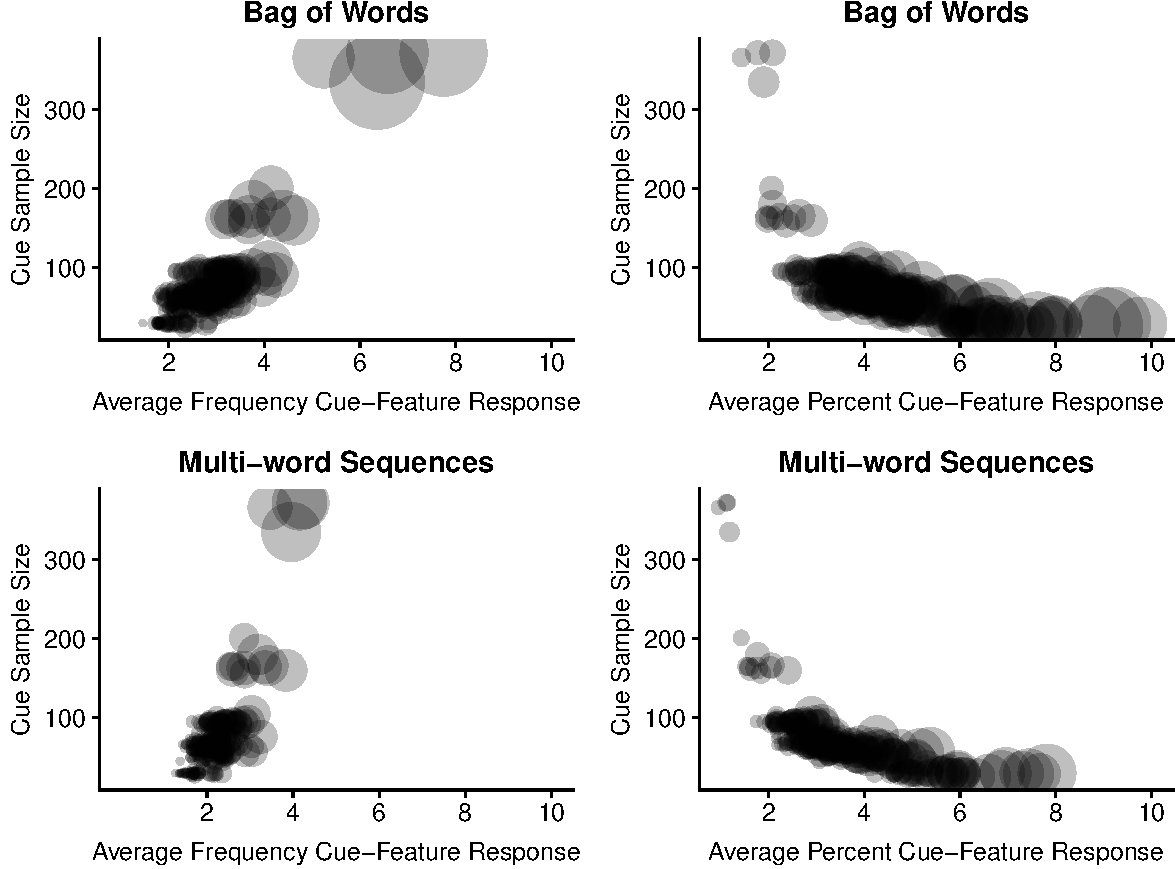
\includegraphics{flt_manuscript_files/figure-latex/correlation-fig-1.pdf}
\caption{\label{fig:correlation-fig}Correlation of sample size with the average cue-feature frequency (left) and percent (right) of response for each cue for both processing approaches. Each point represents a cue word, and the size of the point indicates the variability of the average frequency (left) or percent (right).}
\end{figure}

\hypertarget{internal-comparison-of-approach}{%
\subsection{Internal Comparison of Approach}\label{internal-comparison-of-approach}}

In this section, we show that the bag of words approach matches the data from McRae et al. (2005), Vinson and Vigliocco (2008), and Buchanan et al. (2019), which compares data processed completely through code to datasets that were primarily hand coded. In Buchanan et al. (2019), the McRae et al. (2005) and Vinson and Vigliocco (2008) datasets were recoded in a bag of words approach, and the comparison between all three is provided below. The multi-word sequence approach would be comparable if one or more datasets used the same structured data collection approach or with considerable hand coded rules for feature combinations. The data from open ended responses, such as the Buchanan et al. (2019), could potentially be compared in the demonstrated multi-word sequence approach, if the raw data from other such projects were available.

\begin{table}[t]

\caption{\label{tab:tab7}Cosine Overlap with Previous Data Collection}
\centering
\begin{tabular}{lllll}
\toprule
\multicolumn{1}{c}{ } & \multicolumn{2}{c}{With Stopwords} & \multicolumn{2}{c}{No Stopwords} \\
\cmidrule(l{3pt}r{3pt}){2-3} \cmidrule(l{3pt}r{3pt}){4-5}
Statistic & Original & Translated & Original & Translated\\
\midrule
B Mean & .55 & .58 & .69 & .74\\
B SD & .16 & .16 & .16 & .15\\
M Mean & .33 & .50 & .39 & .59\\
M SD & .15 & .13 & .18 & .13\\
V Mean & .50 & .50 & .60 & .59\\
\addlinespace
V SD & .18 & .18 & .18 & .19\\
\bottomrule
\multicolumn{5}{l}{\textsuperscript{} $Note$. Translated values are hand coded lemmatization from}\\
\multicolumn{5}{l}{Buchanan et al. (2019). B: Buchanan et al. (2019), M: McRae et}\\
\multicolumn{5}{l}{al. (2005), V: Vinson \& Vigliocco (2008). $N$ values are 226,}\\
\multicolumn{5}{l}{61, and 68 respectively.}\\
\end{tabular}
\end{table}

Cosine is often used as a measure of semantic similarity, indicating the feature overlap between two sets of cue-feature lists. These values can range from 0 (no overlap) to 1 (perfect overlap). Two cosine values can be derived from the Buchanan et al. (2019) data: the raw cosine, which included all features as listed and the cosine for lemmatized responses. Each cue in the sample data for this project was compared to the corresponding cue in the Buchanan et al. (2019). If data were processed in an identical fashion, the cosine values would be nearly 1 for Buchanan et al. (2019) data or match the cosine values found for McRae et al. (2005) and Vinson and Vigliocco (2008) in the Buchanan et al. (2019) results: original feature cosine = .54-.55, and lemmatized\footnote{These results were lemmatized by creating a lookup dictionary from the features listed in the Buchanan et al. (2019) norms} features = .66-.67. However, all previous datasets have been reduced by eliminating idiosyncratic features at various points, and therefore, we might expect that noise in the data would reduce the average cosine values. Table \ref{tab:tab7} shows the role of using a cut-off for low-frequent or idiosyncratic responses by calculating the cosine values when using varying cut-offs or stopword filtering. On the left, the cosine values with stopwords are provided for both the original feature listed (i.e., no lemmatization) and the lemmatized features. The right side of the table includes the cosine values once stopwords have been removed. The removal of stopwords increases the match between sets indicating how removing these terms can improve prediction. The cosine values for no stopwords indicate a somewhat comparable set of data, with lower values for McRae et al. (2005) than previous results in the original feature sets. These values indicate that the data processed entirely in \emph{R} produces a comparable set of results, albeit with added noise of small frequency features.

\hypertarget{external-comparison-of-approach}{%
\subsection{External Comparison of Approach}\label{external-comparison-of-approach}}

The MEN dataset (Bruni et al., 2014) contains cue-cue pairs of English words rating for similarity by Amazon Mechanical Turk participants for stimuli taken from the McRae et al. (2005) feature norms. In their rating task, participants were shown two cue-cue pairs and asked to select the more related pair of the two presented. Each pair was rated by 50 participants, and thus, a score of 50 indicates high relatedness, while a score of 0 indicates no relatedness. The ratings for the selected set of cues provided in this analysis was 2 - 49 with an average rating of 25.79 (\emph{SD} = 12.00). The ratings were compared to the cosine calculated between cues using the bag of words method with and without stopwords. The correlation between bag of words cosines with stopwords and the MEN ratings was \(r = .54\), 95\% CI \([.42\), \(.63]\), \emph{N} = 179, indicating agreement between raters and cosine values. The agreement between ratings and bag of word cosine values was higher when stopwords were excluded, \(r = .70\), 95\% CI \([.61\), \(.76]\).

\hypertarget{discussion}{%
\section{Discussion}\label{discussion}}

Semantic feature listing tasks are used across various disciplines and are likely to remain an important source of information about the subjective meaning of concepts. In this article we have outlined a workflow to process large datasets where features consist of unstructured short propositions derived from written language. The advantage to this workflow is two-fold. First, science practices are shifting to open procedures and practices (Nosek et al., 2015), and reproducible research is key (Peng, 2011). Second, automated processing provides faster data analysis than hand-coded systems, and the ability to examine how processing steps affect results. We have shown that the automated procedure provides a comparable set of results to the hand-coded systems from Buchanan et al. (2019), McRae et al. (2005), and Vinson and Vigliocco (2008). The addition of specialized lemmas and other word exclusions (i.e., \textless{}\emph{sometimes}\textgreater{}, \textless{}\emph{usually}\textgreater{}, \textless{}\emph{lot}\textgreater{} or idiosyncratic features) would provide more reduction, and thus, more overlap between hand and automated processing. Further, the automated data processing showed strong correlations with external subjective ratings of cue-cue relatedness in the MEN dataset. We suggest the workflow shown in Figure \ref{fig:flowchart} and the suggested \emph{R} code can provide a framework for researchers to use on their own data.

\hypertarget{extending-the-approach}{%
\subsubsection{Extending the approach}\label{extending-the-approach}}

An attractive property of the subjective feature listing task is that it results in transparent representations. As a result, many researchers have taken additional steps to group specific types of knowledge together, depending on semantic relations (e.g., taxonomy relations) or their mapping onto distinct brain regions (Fairhall \& Caramazza, 2013). Typically this involves applying a hand-crafted coding scheme, which requires a substantial effort. One of the common ontologies is the one developed by Wu and Barsalou (2009). The ontology is structured as a hierarchical taxonomy for coding categories as part of the feature listing task. It has been used in several projects, notably the McRae et al. (2005). Examples of the categories include taxonomic (synonyms, subordinates), entity (internal components, behavior, spatial relations), situation (location, time), and introspective properties (emotion, evaluation). Coding ontology may be best performed systematically with look-up rules of previously decided upon factors, however, clustering analyses may provide a potential avenue to explore categorizing features within the current dataset. One limitation to this method the sheer size of the idiosyncratic features as mentioned above, and thus, features smaller in number may be more difficult to group.

\begin{table}[t]

\caption{\label{tab:tab8}Top Ten Ontology Labels}
\centering
\begin{tabular}{llll}
\toprule
Parts & Function & Location & Category\\
\midrule
brush use & brush hair & scissors cut & flute instrument\\
lawn grass & river water & snow cold & snow white\\
snail shell & branch tree & farm land & elephant animal\\
river stream & chair sit & cabin wood & cabbage green\\
radio music & leaf plant & rocket space & dagger knife\\
\addlinespace
elephant trunk & kitchen food & breakfast day & apple fruit\\
zebra stripe & hammer nail & stone rock & hammer tool\\
river flow & garden flower & bacon pig & lion king\\
door open & oven cook & shoe foot & cabbage vegetable\\
dragon fire & leaf green & toy play & furniture table\\
\bottomrule
\end{tabular}
\end{table}

Potentially, a simple ontology can be mapped using an approach similar to Strudel (structured dimension extraction and labeling, Baroni et al., 2010). Strudel is a corpus-based semantic model wherein cue words are found in a large text corpus and matched to nouns, verbs, and adjectives that appear near a concept. Using specific patterns of expected feature listing, Baroni et al. (2010) were able build a model of English concepts and their properties that aligned with semantic feature production norms. From this model, they were able to cluster properties based on their lexical patterns. For example, if a sentence included the phrase \emph{fruit, such as an apple}, this lexical pattern would be classified as \emph{such\_as+right}, indicating that the concept (apple) was found to the right of the property (fruit) with the phrase such as connecting them. Using clustering, Baroni et al. (2010) was able to assign four ontology labels to properties: part, category, location, and function. Using these results, we can match 2279 of the bag of words features (5\%). These features were predominately parts (39.7), followed by function (30.7), location (24.2), and category (5.4). Table \ref{tab:tab8} indicates ten of the most frequent cue-feature pairs for each ontology label, excluding duplicate features across cues. An examination of the top results indicates coherent labels (parts: ZEBRA \textless{}\emph{stripe}\textgreater{}, location: SHOE \textless{}\emph{foot}\textgreater{}, and category: FURNITURE \textless{}\emph{table}\textgreater{}); however, there are also a few mismatches (location: SCISSORS \textless{}\emph{cut}\textgreater{}, function: LEAF \textless{}\emph{green}\textgreater{}). This model represents an area in which one might begin to automate the labeling process, likely combined with other pre-defined rule sets.

\hypertarget{some-limitations}{%
\subsubsection{Some limitations}\label{some-limitations}}

So far we have not investigated to what extend the automatic procedure leads to equally good representations for different types of concepts. More specifically, abstract concepts tend to have a larger number of features, and especially for these types of concepts, pooling together features might improve the quality of the final representation. Potentially, this might require additional steps in which features are not only grouped based on surface properties but might also benefit from grouping synonymous words. Within this framework, the properties could be added within a lookup dictionary to further promote an open and transparent coding for data processing.

\newpage

\hypertarget{references}{%
\section{References}\label{references}}

\begingroup
\setlength{\parindent}{-0.5in}
\setlength{\leftskip}{0.5in}

\hypertarget{refs}{}
\leavevmode\hypertarget{ref-Baroni2010}{}%
Baroni, M., Murphy, B., Barbu, E., \& Poesio, M. (2010). Strudel: A corpus-based semantic model based on properties and types. \emph{Cognitive Science}, \emph{34}(2), 222--254. doi:\href{https://doi.org/10.1111/j.1551-6709.2009.01068.x}{10.1111/j.1551-6709.2009.01068.x}

\leavevmode\hypertarget{ref-Benoit2017}{}%
Benoit, K., Muhr, D., \& Watanabe, K. (2017). stopwords: Multilingual stopword lists. Retrieved from \url{https://cran.r-project.org/web/packages/stopwords/index.html}

\leavevmode\hypertarget{ref-Bruni2014}{}%
Bruni, E., Tran, N. K., \& Baroni, M. (2014). Multimodal distributional semantics. \emph{Journal of Artificial Intelligence Research}, \emph{49}, 1--47. doi:\href{https://doi.org/10.1613/jair.4135}{10.1613/jair.4135}

\leavevmode\hypertarget{ref-Brysbaert2014}{}%
Brysbaert, M., Warriner, A. B., \& Kuperman, V. (2014). Concreteness ratings for 40 thousand generally known English word lemmas. \emph{Behavior Research Methods}, \emph{46}(3), 904--911. doi:\href{https://doi.org/10.3758/s13428-013-0403-5}{10.3758/s13428-013-0403-5}

\leavevmode\hypertarget{ref-Buchanan2013}{}%
Buchanan, E. M., Holmes, J. L., Teasley, M. L., \& Hutchison, K. A. (2013). English semantic word-pair norms and a searchable Web portal for experimental stimulus creation. \emph{Behavior Research Methods}, \emph{45}(3), 746--757. doi:\href{https://doi.org/10.3758/s13428-012-0284-z}{10.3758/s13428-012-0284-z}

\leavevmode\hypertarget{ref-Buchanan2019}{}%
Buchanan, E. M., Valentine, K. D., \& Maxwell, N. P. (2019). English semantic feature production norms: An extended database of 4436 concepts. \emph{Behavior Research Methods}. doi:\href{https://doi.org/10.3758/s13428-019-01243-z}{10.3758/s13428-019-01243-z}

\leavevmode\hypertarget{ref-Caramazza1988}{}%
Caramazza, A., Laudanna, A., \& Romani, C. (1988). Lexical access and inflectional morphology. \emph{Cognition}, \emph{28}(3), 297--332. doi:\href{https://doi.org/10.1016/0010-0277(88)90017-0}{10.1016/0010-0277(88)90017-0}

\leavevmode\hypertarget{ref-Catricala2015}{}%
Catricalà, E., Della Rosa, P. A., Plebani, V., Perani, D., Garrard, P., \& Cappa, S. F. (2015). Semantic feature degradation and naming performance. Evidence from neurodegenerative disorders. \emph{Brain and Language}, \emph{147}, 58--65. doi:\href{https://doi.org/10.1016/J.BANDL.2015.05.007}{10.1016/J.BANDL.2015.05.007}

\leavevmode\hypertarget{ref-Collins1969}{}%
Collins, A. M., \& Quillian, M. R. (1969). Retrieval time from semantic memory. \emph{Journal of Verbal Learning and Verbal Behavior}, \emph{8}(2), 240--247. doi:\href{https://doi.org/10.1016/S0022-5371(69)80069-1}{10.1016/S0022-5371(69)80069-1}

\leavevmode\hypertarget{ref-Cree2003}{}%
Cree, G. S., \& McRae, K. (2003). Analyzing the factors underlying the structure and computation of the meaning of chipmunk, cherry, chisel, cheese, and cello (and many other such concrete nouns). \emph{Journal of Experimental Psychology: General}, \emph{132}(2), 163--201. doi:\href{https://doi.org/10.1037/0096-3445.132.2.163}{10.1037/0096-3445.132.2.163}

\leavevmode\hypertarget{ref-DanieleZannino2006}{}%
Daniele Zannino, G., Perri, R., Pasqualetti, P., Caltagirone, C., \& Carlesimo, G. A. (2006). Analysis of the semantic representations of living and nonliving concepts: a normative study. \emph{Cognitive Neuropsychology}, \emph{23}(4), 515--540.

\leavevmode\hypertarget{ref-DeDeyne2008c}{}%
De Deyne, S., \& Storms, G. (2008). Word associations: Norms for 1,424 Dutch words in a continuous task. \emph{Behavior Research Methods}, \emph{40}(1), 198--205. doi:\href{https://doi.org/10.3758/BRM.40.1.198}{10.3758/BRM.40.1.198}

\leavevmode\hypertarget{ref-DeQueiroz2019}{}%
De Queiroz, G., Hvitfeldt E, Keyes O, Misra K, Mastny T, Erickson J, \ldots{} Silge J. (2019). tidytext: Text mining using 'dplyr', 'ggplot2', and other tidy tools. Retrieved from \url{https://cran.r-project.org/web/packages/tidytext/index.html}

\leavevmode\hypertarget{ref-Devereux2014}{}%
Devereux, B. J., Tyler, L. K., Geertzen, J., \& Randall, B. (2014). The Centre for Speech, Language and the Brain (CSLB) concept property norms. \emph{Behavior Research Methods}, \emph{46}(4), 1119--1127. doi:\href{https://doi.org/10.3758/s13428-013-0420-4}{10.3758/s13428-013-0420-4}

\leavevmode\hypertarget{ref-Fairhall2013}{}%
Fairhall, S. L., \& Caramazza, A. (2013). Category-selective neural substrates for person- and place-related concepts. \emph{Cortex}, \emph{49}(10), 2748--2757. doi:\href{https://doi.org/10.1016/j.cortex.2013.05.010}{10.1016/j.cortex.2013.05.010}

\leavevmode\hypertarget{ref-Farah1991}{}%
Farah, M. J., \& McClelland, J. L. (1991). A computational model of semantic memory impairment: Modality specificity and emergent category specificity. \emph{Journal of Experimental Psychology: General}, \emph{120}(4), 339--357. doi:\href{https://doi.org/10.1037/0096-3445.120.4.339}{10.1037/0096-3445.120.4.339}

\leavevmode\hypertarget{ref-Gagolewski2019}{}%
Gagolewski, M., \& Tartanus, B. (2019). stringi: Character string processing facilities. Retrieved from \url{https://cran.r-project.org/web/packages/stringi/index.html}

\leavevmode\hypertarget{ref-Garrard2001}{}%
Garrard, P., Lambon Ralph, M. A., Hodges, J. R., \& Patterson, K. (2001). Prototypicality, distinctiveness, and intercorrelation: Analyses of the semantic attributes of living and nonliving concepts. \emph{Cognitive Neuropsychology}, \emph{18}(2), 125--174. doi:\href{https://doi.org/10.1080/02643290125857}{10.1080/02643290125857}

\leavevmode\hypertarget{ref-Humphreys2001}{}%
Humphreys, G. W., \& Forde, E. M. (2001). Hierarchies, similarity, and interactivity in object recognition: "category-specific" neuropsychological deficits. \emph{The Behavioral and Brain Sciences}, \emph{24}(3), 453--476.

\leavevmode\hypertarget{ref-Jackendoff}{}%
Jackendoff, R. (1990). On Larson's treatment of the double object construction. The MIT Press. doi:\href{https://doi.org/10.2307/4178683}{10.2307/4178683}

\leavevmode\hypertarget{ref-Jackendoff1992}{}%
Jackendoff, R. (1992). \emph{Semantic structures}. Boston, MA: MIT Press.

\leavevmode\hypertarget{ref-Kremer2011a}{}%
Kremer, G., \& Baroni, M. (2011). A set of semantic norms for German and Italian. \emph{Behavior Research Methods}, \emph{43}(1), 97--109. doi:\href{https://doi.org/10.3758/s13428-010-0028-x}{10.3758/s13428-010-0028-x}

\leavevmode\hypertarget{ref-Lebani2016}{}%
Lebani, G. E., Lenci, A., \& Bondielli, A. (2016). You are what you do: An empirical characterization of the semantic content of the thematic roles for a group of Italian verbs. \emph{Journal of Cognitive Science}, \emph{16}(4), 401--430. doi:\href{https://doi.org/10.17791/jcs.2015.16.4.401}{10.17791/jcs.2015.16.4.401}

\leavevmode\hypertarget{ref-Lenci2013}{}%
Lenci, A., Baroni, M., Cazzolli, G., \& Marotta, G. (2013). BLIND: A set of semantic feature norms from the congenitally blind. \emph{Behavior Research Methods}, \emph{45}(4), 1218--1233. doi:\href{https://doi.org/10.3758/s13428-013-0323-4}{10.3758/s13428-013-0323-4}

\leavevmode\hypertarget{ref-Marques2007a}{}%
Marques, J. F., Fonseca, F. L., Morais, S., \& Pinto, I. A. (2007). Estimated age of acquisition norms for 834 Portuguese nouns and their relation with other psycholinguistic variables. \emph{Behavior Research Methods}, \emph{39}(3), 439--444. doi:\href{https://doi.org/10.3758/BF03193013}{10.3758/BF03193013}

\leavevmode\hypertarget{ref-McRae2005}{}%
McRae, K., Cree, G. S., Seidenberg, M. S., \& McNorgan, C. (2005). Semantic feature production norms for a large set of living and nonliving things. \emph{Behavior Research Methods}, \emph{37}(4), 547--559. doi:\href{https://doi.org/10.3758/BF03192726}{10.3758/BF03192726}

\leavevmode\hypertarget{ref-Michalke2018}{}%
Michalke, M. (2018). koRpus: An R package for text analysis. Retrieved from \url{https://cran.r-project.org/web/packages/koRpus/index.html}

\leavevmode\hypertarget{ref-Minsky1975}{}%
Minsky, M. (1975). A framework for representing knowledge. In P. H. Winston (Ed.), \emph{The psychology of computer vision} (pp. 211--277). Winston, NY: McGraw Hill.

\leavevmode\hypertarget{ref-Montefinese2019}{}%
Montefinese, M. (2019). Semantic representation of abstract and concrete words: a minireview of neural evidence. \emph{Journal of Neurophysiology}, \emph{121}(5), 1585--1587. doi:\href{https://doi.org/10.1152/jn.00065.2019}{10.1152/jn.00065.2019}

\leavevmode\hypertarget{ref-Montefinese2013}{}%
Montefinese, M., Ambrosini, E., Fairfield, B., \& Mammarella, N. (2013). Semantic memory: A feature-based analysis and new norms for Italian. \emph{Behavior Research Methods}, \emph{45}(2), 440--461. doi:\href{https://doi.org/10.3758/s13428-012-0263-4}{10.3758/s13428-012-0263-4}

\leavevmode\hypertarget{ref-Montefinese2014}{}%
Montefinese, M., Ambrosini, E., Fairfield, B., \& Mammarella, N. (2014). Semantic significance: a new measure of feature salience. \emph{Memory \& Cognition}, \emph{42}(3), 355--369. doi:\href{https://doi.org/10.3758/s13421-013-0365-y}{10.3758/s13421-013-0365-y}

\leavevmode\hypertarget{ref-Montefinese2015}{}%
Montefinese, M., Zannino, G. D., \& Ambrosini, E. (2015). Semantic similarity between old and new items produces false alarms in recognition memory. \emph{Psychological Research}, \emph{79}(5), 785--794. doi:\href{https://doi.org/10.1007/s00426-014-0615-z}{10.1007/s00426-014-0615-z}

\leavevmode\hypertarget{ref-Norman1975}{}%
Norman, D. A., \& Rumelhart, D. E. (1975). \emph{Explorations in cognition}. San Francisco, CA: Freeman.

\leavevmode\hypertarget{ref-Nosek2015}{}%
Nosek, B. A., Alter, G., Banks, G. C., Borsboom, D., Bowman, S. D., Breckler, S. J., \ldots{} Yarkoni, T. (2015). Promoting an open research culture. \emph{Science}, \emph{348}(6242), 1422--1425. doi:\href{https://doi.org/10.1126/science.aab2374}{10.1126/science.aab2374}

\leavevmode\hypertarget{ref-Ooms2018}{}%
Ooms, J. (2018). The hunspell package: High-Performance Stemmer, Tokenizer, and Spell Checker for R. Retrieved from \url{https://cran.r-project.org/web/packages/hunspell/}

\leavevmode\hypertarget{ref-Peng2011}{}%
Peng, R. D. (2011). Reproducible research in computational science. \emph{Science (New York, N.Y.)}, \emph{334}(6060), 1226--7. doi:\href{https://doi.org/10.1126/science.1213847}{10.1126/science.1213847}

\leavevmode\hypertarget{ref-Pexman2008}{}%
Pexman, P. M., Hargreaves, I. S., Siakaluk, P. D., Bodner, G. E., \& Pope, J. (2008). There are many ways to be rich: Effects of three measures of semantic richness on visual word recognition. \emph{Psychonomic Bulletin \& Review}, \emph{15}(1), 161--167. doi:\href{https://doi.org/10.3758/PBR.15.1.161}{10.3758/PBR.15.1.161}

\leavevmode\hypertarget{ref-Plaut2002}{}%
Plaut, D. C. (2002). Graded modality-specific specialisation in semantics: A computational account of optic aphasia. \emph{Cognitive Neuropsychology}, \emph{19}(7), 603--639. doi:\href{https://doi.org/10.1080/02643290244000112}{10.1080/02643290244000112}

\leavevmode\hypertarget{ref-Recchia2012}{}%
Recchia, G., \& Jones, M. N. (2012). The semantic richness of abstract concepts. \emph{Frontiers in Human Neuroscience}, \emph{6}, 315. doi:\href{https://doi.org/10.3389/fnhum.2012.00315}{10.3389/fnhum.2012.00315}

\leavevmode\hypertarget{ref-Rogers2004}{}%
Rogers, T. T., Lambon Ralph, M. A., Garrard, P., Bozeat, S., McClelland, J. L., Hodges, J. R., \& Patterson, K. (2004). Structure and deterioration of semantic memory: A neuropsychological and computational investigation. \emph{Psychological Review}, \emph{111}(1), 205--235. doi:\href{https://doi.org/10.1037/0033-295X.111.1.205}{10.1037/0033-295X.111.1.205}

\leavevmode\hypertarget{ref-Rosch1975}{}%
Rosch, E., \& Mervis, C. B. (1975). Family resemblances: Studies in the internal structure of categories. \emph{Cognitive Psychology}, \emph{7}(4), 573--605. doi:\href{https://doi.org/10.1016/0010-0285(75)90024-9}{10.1016/0010-0285(75)90024-9}

\leavevmode\hypertarget{ref-Ruts2004}{}%
Ruts, W., De Deyne, S., Ameel, E., Vanpaemel, W., Verbeemen, T., \& Storms, G. (2004). Dutch norm data for 13 semantic categories and 338 exemplars. \emph{Behavior Research Methods, Instruments, \& Computers}, \emph{36}(3), 506--515. doi:\href{https://doi.org/10.3758/BF03195597}{10.3758/BF03195597}

\leavevmode\hypertarget{ref-Saffran1999}{}%
Saffran, E., \& Sholl, A. (1999). Clues to the function and neural architecture of word meaning. In P. Hogoort \& C. Brown (Eds.), \emph{The neurocognition of language}. Oxford University Press.

\leavevmode\hypertarget{ref-Santos2011}{}%
Santos, A., Chaigneau, S. E., Simmons, W. K., \& Barsalou, L. W. (2011). Property generation reflects word association and situated simulation. \emph{Language and Cognition}, \emph{3}(1), 83--119. doi:\href{https://doi.org/10.1515/langcog.2011.004}{10.1515/langcog.2011.004}

\leavevmode\hypertarget{ref-Sartori2004}{}%
Sartori, G., \& Lombardi, L. (2004). Semantic relevance and semantic disorders. \emph{Journal of Cognitive Neuroscience}, \emph{16}(3), 439--452. doi:\href{https://doi.org/10.1162/089892904322926773}{10.1162/089892904322926773}

\leavevmode\hypertarget{ref-Schmid1994}{}%
Schmid, H. (1994). Probabilistic part of speech tagging using decision trees. doi:\href{https://doi.org/10.1.1.28.1139}{10.1.1.28.1139}

\leavevmode\hypertarget{ref-Smith1974}{}%
Smith, E. E., Shoben, E. J., \& Rips, L. J. (1974). Structure and process in semantic memory: A featural model for semantic decisions. \emph{Psychological Review}, \emph{81}(3), 214--241. doi:\href{https://doi.org/10.1037/h0036351}{10.1037/h0036351}

\leavevmode\hypertarget{ref-Smith1981}{}%
Smith, E., \& Medin, D. L. (1981). \emph{Categories and concepts (Vol. 9)}. Cambridge, MA: Harvard University Press.

\leavevmode\hypertarget{ref-Ushey2018}{}%
Ushey, K., McPherson, J., Cheng, J., Atkins, A., \& Allaire, J. (2018). packrat: A dependency management system for projects and their R rackage dependencies. Retrieved from \url{https://cran.r-project.org/web/packages/packrat/index.html}

\leavevmode\hypertarget{ref-Vigliocco2004}{}%
Vigliocco, G., Vinson, D. P., Lewis, W., \& Garrett, M. F. (2004). Representing the meanings of object and action words: The featural and unitary semantic space hypothesis. \emph{Cognitive Psychology}, \emph{48}(4), 422--488. doi:\href{https://doi.org/10.1016/j.cogpsych.2003.09.001}{10.1016/j.cogpsych.2003.09.001}

\leavevmode\hypertarget{ref-Vinson2008}{}%
Vinson, D. P., \& Vigliocco, G. (2008). Semantic feature production norms for a large set of objects and events. \emph{Behavior Research Methods}, \emph{40}(1), 183--190. doi:\href{https://doi.org/10.3758/BRM.40.1.183}{10.3758/BRM.40.1.183}

\leavevmode\hypertarget{ref-Vivas2017}{}%
Vivas, J., Vivas, L., Comesaña, A., Coni, A. G., \& Vorano, A. (2017). Spanish semantic feature production norms for 400 concrete concepts. \emph{Behavior Research Methods}, \emph{49}(3), 1095--1106. doi:\href{https://doi.org/10.3758/s13428-016-0777-2}{10.3758/s13428-016-0777-2}

\leavevmode\hypertarget{ref-Wickham2019}{}%
Wickham, H., Francios, R., Henry, L., Muller, K., \& Rstudio. (2019). dplyr: A grammar of data manipulation. Retrieved from \url{https://cloud.r-project.org/web/packages/dplyr/index.html}

\leavevmode\hypertarget{ref-KatjaWiemer-Hastings2005}{}%
Wiemer-Hastings, K., \& Xu, X. (2005). Content differences for abstract and concrete concepts. \emph{Cognitive Science}, \emph{29}(5), 719--736. doi:\href{https://doi.org/10.1207/s15516709cog0000_33}{10.1207/s15516709cog0000\_33}

\leavevmode\hypertarget{ref-Wu2009}{}%
Wu, L.-l., \& Barsalou, L. W. (2009). Perceptual simulation in conceptual combination: Evidence from property generation. \emph{Acta Psychologica}, \emph{132}(2), 173--189. doi:\href{https://doi.org/10.1016/j.actpsy.2009.02.002}{10.1016/j.actpsy.2009.02.002}

\leavevmode\hypertarget{ref-Zannino2006}{}%
Zannino, G. D., Perri, R., Pasqualetti, P., Caltagirone, C., \& Carlesimo, G. A. (2006). (Category-specific) semantic deficit in Alzheimer's patients: The role of semantic distance. \emph{Neuropsychologia}, \emph{44}(1), 52--61. doi:\href{https://doi.org/10.1016/J.NEUROPSYCHOLOGIA.2005.04.008}{10.1016/J.NEUROPSYCHOLOGIA.2005.04.008}

\endgroup


\end{document}
